\section{Information Theory}%
\label{sec:information-theory}
\vspace{1cm}
\begin{figure}[h!]%
	\label{fig:info}
	\centering
	\fcolorbox{black}{white}{\includegraphics[width=0.3\textwidth]{entropy}}
	\caption{Visual representation of entropy as a measure of uncertainty in information systems. Source: \href{https://www.consciousentities.com/2017/02/consciousness-entropy/}{Conscious Entities, Peter Hankins}}
\end{figure}
\vspace{1cm}
\noindent Information theory emerged as a formal discipline in 1948 with Claude Shannon's seminal publication \textit{A Mathematical Theory of Communication}. Shannon's work was influenced by earlier research in thermodynamics by Boltzmann and Gibbs, as well as contributions from Hartley and Nyquist at Bell Laboratories~\cite{ref:losee-1997}. While many aspects of information theory—including compression algorithms, coding schemes, and data transmission over noisy channels—fall beyond the scope of this thesis, certain information-theoretic quantities play a crucial role in machine learning and warrant detailed discussion.

\begin{remark}
	The information we discuss here specifically concerns the probability distribution over elementary outcomes, rather than the semantic content of those outcomes. The significance of probability lies in its ability to quantify our certainty when making inferences. The most valuable information in this context is contained within the probability distribution itself.
\end{remark}

Information theory provides powerful tools for analyzing deep learning systems. When we conceptualize neural networks as noisy communication channels, the relevance of information theory becomes particularly evident. As Mackay observed in~\cite{ref:mackay-2003}, ``brains are the ultimate compression and communication systems. And the state-of-the-art algorithms for both data compression and error-correcting codes use the same tools as machine learning''. He further anticipated that ``the best data compression algorithms will result from the development of artificial intelligence methods''.

The most fundamental concept in information theory is entropy. Before presenting its formal definition, we will motivate entropy as a measure of uncertainty by systematically deriving it from first principles. We begin by defining a function $\eta$ as a measure of uncertainty and then derive entropy based on the requirements this function must satisfy.

\begin{definition}
	Let $(\mathcal{X}, p)$ be a discrete probability space. We define
	\textnormal{\sffamily uncertainty} as a real-valued function
	$\eta(\cdot): \mathcal{X} \mapsto \mathbb{R}^+$ that depends only on the
	probabilities of elementary outcomes and satisfies the following conditions:
	\begin{enumerate}[(i)]
		\item If an outcome $x$ is certain to occur, there is no uncertainty about it, and thus $\eta(x) = 0$;
		\item For any two outcomes $x$, $x^\prime$, we have $p(x) < p(x^\prime) \iff
			      \eta(x) > \eta(x^\prime)$;
		\item For any two independent outcomes $x$, $x^\prime$, the
		      uncertainty of their joint occurrence equals the sum of their
		      individual uncertainties, i.e.,
		      $\eta(x \cdot x^\prime) = \eta(x) + \eta(x^\prime)$.
	\end{enumerate}
\end{definition}
\begin{remark}
	This definition adapts the framework presented by~\cite{ref:martin-2011}.
\end{remark}

It is intuitive that new information reduces uncertainty. Common outcomes provide less information than rare ones, suggesting that $\eta$ should be inversely proportional to the probability of the outcome:
\begin{align}
	\label{eq:eta-1}
	\eta(x) \propto {1 \over p(x)}
\end{align}

Given that $\eta$ must satisfy $\eta(x \cdot x^\prime) = \eta(x) + \eta(x^\prime)$, we must define $\eta$ in terms of a logarithm. This is necessary because the probability of two independent outcomes is the product of their individual probabilities, whereas we require information to be additive. Therefore:
\begin{align}
	\label{eq:eta-3}
	\eta(x) \approx \log{1 \over p(x)}.
\end{align}

For probability distributions, we need a measure of uncertainty that quantifies the average uncertainty contained in $(\mathcal{X}, p)$. This requires weighting the calculation by the probability of observing each outcome. Thus, we seek a measure on the probability distribution over $\mathcal{X}$. We adjust our notation, using the capital eta (resembling the Latin H), to define:
\begin{align}
	\label{eq:eta-almost}
	H(p) = \sum_{x \in \mathcal{X}} p(x) \log{1 \over p(x)}.
\end{align}

This defines entropy as a measure of the average amount of surprise associated with outcomes from $(\mathcal{X}, p)$. Entropy reaches its maximum when we cannot predict outcomes with any confidence, which occurs when probabilities are uniformly distributed across all possible outcomes:
\begin{align}
	\label{eq:eta-2}
	H(p) \leq \log{|\mathcal{X}|}
\end{align}

We can also interpret entropy as the amount of information, measured in binary units (bits), required to describe outcomes drawn from $(\mathcal{X}, p)$. This interpretation follows from the fact that the logarithm indicates how many bits we need to encode this uncertainty:
\begin{align}
	\label{eq:understand-log}
	\log_2{1 \over p(x)} = n \iff 2^n = {1 \over p(x)}.
\end{align}
Although base-2 logarithms are common in information theory, any base (including $e$ and 10) can be used depending on the application.

\begin{definition}
	Let $(\mathcal{X}, p)$ be a discrete probability space. The \textnormal{\sffamily
		entropy} of a probability distribution $p$ with mass function $p$, denoted
	by $H(p)$, is the average amount of uncertainty associated with elementary outcomes
	from $(\mathcal{X}, p)$. We write:
	\begin{align}
		\label{eq:entropy}
		H(p) = - \mathbb{E}_{x \sim p} \left[ \log{p(x)} \right].
	\end{align}
	The entropy of a probability distribution quantifies the expected variation in samples drawn from $(\mathcal{X}, p)$. The uniform distribution maximizes entropy since all outcomes are equally surprising.
\end{definition}

Figure~\ref{fig:entropy-coin-toss} illustrates the entropy of a probability distribution over two states as a function of the distribution's symmetry. As the probability of heads $p(H)$ approaches 0 or 1, uncertainty vanishes, while uncertainty is maximized when probability is equally distributed between heads and tails.

\begin{figure}[H]
	\centering
	\begin{tikzpicture}
		\begin{axis}[
				ymin = 0,
				ymax = 1,
				xmin = 0,
				xmax = 1,
				xlabel = $p(H)$,
				ylabel = $H(p)$,
				enlargelimits = false]
			\addplot [samples = 300, blue] {-x*log2(x)-(1-x)*log2(1-x)};
		\end{axis}
	\end{tikzpicture}
	\caption{Entropy of a coin toss as a function of the symmetry of $p(H)$.}%
	\label{fig:entropy-coin-toss}
\end{figure}

\begin{example}
	The entropy of a fair coin toss is 1 bit, while the entropy of $m$ independent tosses is $m$ bits. For a system with two equally probable states, we need 1 bit to represent the outcome, whereas for three equally probable states, we need approximately 1.585 bits.
\end{example}

\subsubsection*{Entropy-based Quantities}

To establish a clear distinction between metrics and divergences, we first define a metric:

\begin{definition}
	A \textnormal{\sffamily metric} on a set $\mathcal{X}$ is a function $d(\cdot, \cdot): \mathcal{X} \times
		\mathcal{X} \mapsto \mathbb{R}^+$ such that, $\forall x, y, z \in \mathcal{X}$:
	\begin{enumerate}
		\item $d(x, y) \geq 0$, and $d(x, y) = 0 \iff x = y$
		\item $d(x, y) = d(y, x)$
		\item $d(x, z) \leq d(x, y) + d(y, z)$ (triangle inequality)
	\end{enumerate}
\end{definition}

\begin{remark}
	A divergence is a weaker concept than a distance. A divergence need not be symmetric nor satisfy the triangle inequality.
\end{remark}

\begin{definition}
	Let $\mathcal{P}$ be a space of probability distributions over a finite set $\mathcal{X}$
	such that all $P \in \mathcal{P}$ have the same support. A \textnormal{\sffamily
		divergence} on $\mathcal{P}$ is a function, $\mathbb{D}[\cdot \| \cdot]: \mathcal{P} \times \mathcal{P}
		\mapsto \mathbb{R}^+$, such that $\forall p, q \in \mathcal{P}$:
	\begin{enumerate}[(i)]
		\item $\mathbb{D}[p \| q] \geq 0$
		\item $\mathbb{D}[p \| q] = 0 \iff p = q$.
	\end{enumerate}
\end{definition}

\begin{definition}%
	\label{def:kl-divergence}
	The \textnormal{\sffamily Kullback-Leibler divergence} measures how
	one probability distribution differs from a second, reference probability distribution.
	Also known as \textnormal{\sffamily relative entropy}, \textnormal{\sffamily directed divergence},
	\textnormal{\sffamily information gain}, or \textnormal{\sffamily
		discrimination information}, it is defined as:
	\begin{align}
		\label{eq:KL}
		\mathbb{D}_{KL}[p \| q] = \sum_{x \in \mathcal{X}} p(x) \log{p(x) \over q(x)}.
	\end{align}
	If $p$ and $q$ have the same support, then $\mathbb{D}_{KL}[p \| q] = 0$ if and
	only if $p = q$.
\end{definition}

\begin{remark}
	The Kullback-Leibler divergence is defined only if $p$ is absolutely
	continuous with respect to $q$, i.e., $\forall x$,
	$q(x) = 0 \implies p(x) = 0$. When $p(x) = 0$, the corresponding term in the sum is 0 since $\lim_{x \to 0} x\log{x} = 0$.
\end{remark}

\begin{theorem}
	For a closed convex set $E \subset \mathcal{P}$, where $\mathcal{P}$ is the space of
	all probability distributions over a finite set $\mathcal{X}$, and for a
	distribution $Q \not \in E$, let $P^* \in E$ be defined by
	$p^* = \argmin_{P \in E} \mathbb{D}_{KL}[p \| q]$. Then:
	\begin{align}
		\mathbb{D}_{KL}[p \| q] \geq \mathbb{D}_{KL}[p \| p^*] + \mathbb{D}_{KL}[p^* \| q].
	\end{align}
	The interested reader can consult Theorem 11.6.1 in~\cite{ref:cover-thomas}.
\end{theorem}

\begin{remark}
	The Kullback-Leibler divergence relates to the log-likelihood ratio test used in statistical model comparison. Specifically, $\mathbb{D}_{KL}[p \| q]$ represents the average log-likelihood ratio test with respect to probabilities defined by $p$. For two models $p(x) = f(x|\theta)$ and $q(x) = f(x|\phi)$, the log-likelihood ratio test is:
	\begin{align}
		\lambda(x) & = \log{\prod_{x \in \mathcal{X}} p(x) \over \prod_{x \in \mathcal{X}} q(x)} \\
		           & = \log \prod_{x \in \mathcal{X}} {p(x) \over q(x)}                          \\
		           & = \sum_{x \in \mathcal{X}} \log {p(x) \over q(x)}
	\end{align}
	and its average with respect to $p$ is:
	\begin{align}
		\mathbb{E}_{x \sim p}[\lambda(x)] = \sum_{x \in \mathcal{X}} p(x)\log {p(x) \over q(x)}.
	\end{align}
\end{remark}

This connection to statistical testing provides insight into GAN training. We can view GAN training as fitting $D$ and $G$ to the data via optimizing a goodness-of-fit test, since:
\begin{align}
	\min_\phi\max_\theta{1 \over n} \sum_{i=1}^n \log{D(x_i)} + {1
	\over n} \sum_{i=1}^n\log{(1 - D(G(z_i)))}
\end{align}
has the same fixed point as:
\begin{align}
	 & \min_\phi\max_\theta{1 \over n} \sum_{i=1}^n \left[\log{D(x_i)} - \log{(D(G(z_i)))}\right] \\
	 & = \min_\phi\max_\theta{1 \over n} \sum_{i=1}^n \log{\left({D(x_i) \over D(G(z_i))}\right)}
\end{align}
which represents the Kullback-Leibler divergence or the average log-likelihood ratio test. Since $\forall x$, $D(x) \in [0, 1]$, when $D$ is optimized, it will assign higher probability to real data $x$ than to generated data $G(z)$.

The term \textit{information gain} refers to one interpretation of the Kullback-Leibler divergence. Specifically, $\mathbb{D}_{KL}[p \| q]$ quantifies the information gained about the data when using $q$ as a model instead of $p$. Equivalently, it represents the information lost when $q$ is used to approximate $p$.

\begin{definition}
	The \textnormal{\sffamily reverse Kullback-Leibler divergence} is the asymmetric counterpart:
	\begin{align}
		\label{eq:reverse-KL}
		\mathbb{D}_{KL}[q \| p] = \sum_{x \in \mathcal{X}} q(x) \log{q(x) \over p(x)}.
	\end{align}
	The reverse Kullback-Leibler divergence is the average of the log-likelihood
	ratio test taken with respect to the model $q(x)$:
	\begin{align}
		\mathbb{E}_{x \sim q}[\lambda(x)] = \sum_{x \in \mathcal{X}} q(x)\log {q(x) \over p(x)}.
	\end{align}
\end{definition}

Minimizing the reverse Kullback-Leibler divergence is not equivalent to maximum likelihood methods.

The Kullback-Leibler divergence relates to another quantity frequently used in machine learning: cross entropy.

\begin{definition}
	The \textnormal{\sffamily cross entropy} of $p$ and $q$ (for a given data set) quantifies the total
	uncertainty incurred by modeling the data with $q$ rather than $p$:
	\begin{align}
		H(p, q) = - \sum_{x \in \mathcal{X}} p(x) \log q(x) = -\mathbb{E}_{x \sim p}\left[\log{q(x)}\right].
	\end{align}
\end{definition}

\begin{lemma}
	The cross entropy of $p$ and $q$ equals the sum of the entropy of $p$ and the
	Kullback-Leibler divergence of $p$ and $q$.
\end{lemma}

\begin{proof}
	\begin{align}
		\label{eq:cross-entropy-alt}
		H(p, q) & = -\sum_{x \in \mathcal{X}} p(x) \log q(x)                                                                                     \\
		        & = -\sum_{x \in \mathcal{X}} p(x) \log p(x) + \sum_{x \in \mathcal{X}} p(x) \log p(x) - \sum_{x \in \mathcal{X}} p(x) \log q(x) \\
		        & = -\sum_{x \in \mathcal{X}} p(x) \log p(x) + \sum_{x \in \mathcal{X}} p(x) \log {p(x) \over q(x)}                              \\
		        & = H(p) + \mathbb{D}_{KL}[p \| q]
	\end{align}
\end{proof}

This relationship reveals that the lower bound for cross entropy is the entropy of the probability distribution $p$ over $\mathcal{X}$. Thus, cross entropy represents the uncertainty induced by assuming an incorrect probability distribution over the data, with the additional uncertainty captured by the Kullback-Leibler divergence. Cross entropy is not symmetric since $H(q, p) = H(q) + \mathbb{D}_{KL}[q \| p]$.

As shown in~\cite{ref:goodfellow-original}, the generator minimizes an approximation of the Jensen-Shannon divergence.

\begin{definition}%
	\label{def:jsd}
	Let $p(x)$ and $q(x)$ be probability distributions over a space $\mathcal{X}$. The \textnormal{\sffany Jensen-Shannon divergence} of
	$p(x)$ and $q(x)$ is a symmetrization of the Kullback-Leibler
	divergence:
	\begin{align}
		\mathbb{D}_{JS}[p \| q] = {1 \over 2} \mathbb{D}_{KL}\left[p \| {p + q \over 2}\right] + {1 \over 2} \mathbb{D}_{KL}\left[q \| {p + q \over 2}\right]
	\end{align}
\end{definition}

\begin{remark}
	The Jensen-Shannon divergence is the average of the Kullback-Leibler
	divergence and the reverse Kullback-Leibler divergence.
\end{remark}

\begin{theorem}
	The square root of the Jensen–Shannon divergence is a metric.
\end{theorem}

\begin{proof}
	See~\cite{ref:endres-2003}.
\end{proof}

\subsubsection*{Mutual Information and other Measures}

Information theory provides measures of dependency between random variables, quantifying how much information one distribution contains about another. The following measures are defined in terms of random variables denoted by uppercase letters such as $X$ and $Y$.

\begin{definition}
	Let $(\mathcal{X}, p)$ and $(\mathcal{Y}, q)$ be finite probability spaces ($\mathcal{X}$ and
	$\mathcal{Y}$ need not be distinct) and consider random variables $X \sim p$ and
	$Y \sim q$ with joint probability mass function $\gamma$ and marginal
	probability mass functions $\pi_p \circ \gamma = p$ and $\pi_q \circ \gamma =
		q$. The \textnormal{\sffamily mutual information} $I(X;Y)$ is the
	Kullback-Leibler divergence of $\gamma$ and the product of $p$ and $q$:
	\begin{align}
		\label{eq:mutual-information}
		I(X; Y) = \sum_{x \in \mathcal{X}}\sum_{y \in \mathcal{Y}}\gamma(x, y) \log{{\gamma(x, y) \over p(x)q(y)}}
	\end{align}
\end{definition}

\begin{theorem}
	If the random variables $X$ and $Y$ are independent, then $\gamma(x,y) =
		p(x)q(y)$ and $I(X; Y) = 0$.
\end{theorem}

\begin{remark}
	Mutual information measures the amount of information contained in one
	probability distribution about another, serving as a useful measure of
	statistical dependence.
\end{remark}

\begin{remark}
	Mutual information can also be defined in terms of conditional entropy:
	\begin{align}
		\label{eq:mutual-information-alt}
		I(X; Y) = H(X) - H(X | Y) = H(Y) - H(Y | X)
	\end{align}
	where $H(X | Y)$ is the conditional entropy of $X$ given that $Y$ has
	occurred. In this form, mutual information represents the information contained in one distribution minus the information remaining when the other distribution is known.
\end{remark}

The relationships between different information-theoretic quantities are visualized in the Venn diagram in Figure~\ref{fig:venn-information}.

\begin{figure}[h!]
	\centering
	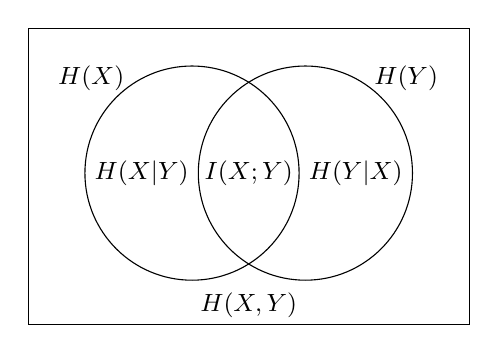
\begin{tikzpicture}[scale=0.8]
		\small
		% Labels
		\draw (0,0) node {$I(X;Y)$};
		\draw (-2.5,1.5) node {$H(X)$};
		\draw (2.5,1.5) node {$H(Y)$};
		\draw (-1.7,0) node {$H(X|Y)$};
		\draw (1.7,0) node {$H(Y|X)$};
		\draw (0,-2.1) node {$H(X,Y)$};
		% Circles
		\draw (-0.9,0) circle (1.7cm);
		\draw (0.9,0) circle (1.7cm);
		% Bounding Rectangle
		\draw (-3.5,-2.4) rectangle (3.5,2.3);
	\end{tikzpicture}
	\caption{Venn Diagram of Information-Theoretic Quantities}%
	\label{fig:venn-information}
\end{figure}

\subsection{Information-Theoretic View of GANs}%
\label{sec:info-value-function}%

We can now analyze the value function $\V = \mathbb{E}_{x \sim p_r}[\log
		D_\theta(x)] + \mathbb{E}_{z \sim p_z}[\log{(1 - D_\theta(G_\phi(z)))}]$ from an information-theoretic perspective. The proposition below considers the behavior at each training step rather than the limiting behavior of $D$ and $G$. Section~\ref{sec:optimization-dynamics} addresses the limiting dynamics between $D$ and $G$.

We claim that GAN training aims to minimize the Kullback-Leibler divergence between the true data distribution $p_r$ and the discriminator's output distribution for real data. Simultaneously, it maximizes the Kullback-Leibler divergence between the generator's prior distribution $p_z$ and the discriminator's output for generated data. Finally, it minimizes the Kullback-Leibler divergence between the generator's prior distribution and the discriminator's assessment of synthetic data.

\begin{remark}
	In this context, the Kullback-Leibler divergence quantifies the additional surprise we experience when observing outcomes from $(\mathcal{X}, p)$ while using an approximation $q$ of the true probability distribution $p$ over $\mathcal{X}$.
\end{remark}

\begin{proposition}%
	\label{thm:info-objective}%
	When considering
	\begin{align}
		\label{eq:consider}
		\min_\phi \max_\theta \mathbb{E}_{x \sim p_r}[\log D_\theta(x)] + \mathbb{E}_{z
		\sim p_z}[\log{(1 - D_\theta(G_\phi(z)))}]
	\end{align}
	from an information-theoretic perspective, the training objectives of the GAN algorithm are to find:
	\begin{enumerate}[(i)]
		\item $\theta \in \Theta$ to minimize $\mathbb{D}_{KL}[p_r \| D(x)]$ and
		      maximize $\mathbb{D}_{KL}[p_z \| D(G(z))]$;
		\item $\phi \in \Phi$ to minimize $\mathbb{D}_{KL}[p_z \| D(G(z))]$.
	\end{enumerate}
\end{proposition}

\begin{proof}
	The first term of $\V$ represents the negative cross entropy of $p_r$ and
	the distribution induced by $D(x)$:
	\begin{align}
		\label{eq:neg-cross-entropy}
		- H(p_r, D) = \sum_{x \in \mathcal{X}}p_r(x)\log(D(x)) = \mathbb{E}_{x \sim p_r} \left[\log(D(x))\right].
	\end{align}
	Since we train the discriminator to maximize
	(\ref{eq:neg-cross-entropy}), this is equivalent to minimizing the cross entropy of $p_r$
	and the distribution induced by $D(x)$. This minimization occurs when the
	Kullback-Leibler divergence of $p_r$ and $p_d$ is 0, since:
	\begin{align}
		H(p_r,D) & = - \sum_{x \in \mathcal{X}} p_r(x) \log p_d(x)                                                                                            \\
		         & = -\sum_{x \in \mathcal{X}} p_r(x) \log p_r(x) + \sum_{x \in \mathcal{X}} p_r(x) \log p_r(x) - \sum_{x \in \mathcal{X}} p_r(x) \log p_d(x) \\
		         & = -\sum_{x \in \mathcal{X}} p_r(x) \log p_r(x) + \sum_{x \in \mathcal{X}} p_r(x) \log {p_r(x) \over
		p_d(x)}                                                                                                                                               \\
		         & = H(p_r) + \mathbb{D}_{KL}[p_r \| D].
	\end{align}
	Since $p_r$ remains fixed during training, the only way to minimize
	$H(p_r,D)$ is to train $D$ to minimize $\mathbb{D}_{KL}[p_r \| D]$, which occurs when
	$p_r = D$. Therefore, when $D$ is optimized, $D(x)$ will return the probability that $x$ was sampled from $p_r$, which equals $p_r(x)$ when $D$ is optimal.

	The second term of (\ref{eq:consider}),
	\begin{align}
		\mathbb{E}_{z \sim p_z}\left[\log(1 - D(G(z)))\right] =
		\sum_{z \sim p_z} p_z(z) \log (1 - D(G(z)))
	\end{align}
	is maximized by $D$, equivalent to $D$ maximizing:
	\begin{align}
		-\sum_{z \sim p_z} p_z(z) \log (D(G(z))),
	\end{align}
	which is the cross entropy of $p_z$ and $D(G(z))$. This means $D$ aims to make $p_z$ and $D(G(z))$ as different as possible. Conversely, given a fixed discriminator $D$, we train $G$ to minimize the same expression, which is equivalent to minimizing:
	\begin{align}
		-\sum_{z \sim p_z} p_z(z) \log (D(G(z)))
	\end{align}
	the cross entropy of $p_z$ and $D(G(z))$.
\end{proof}

The interpretation of this proposition is that the generator aims to make the discriminator's decisions on generated data as uninformative as random noise. The discriminator, meanwhile, seeks to make its decision distribution over training data match the true data distribution, while simultaneously making its decisions on generated data more informative than noise.

Next, we examine the optimization steps as dynamics between approximating and minimizing a divergence.

\subsection{Optimization Dynamics}%
\label{sec:optimization-dynamics}

While Section~\ref{sec:derivation} discussed training $D$ and $G$ from a game-theoretic perspective, we now analyze these results more rigorously with detailed calculations. Throughout this section, we use the following notation: Let $\mathcal{X}$ be our data space and $p_r$ the true probability distribution over $\mathcal{X}$. Let $\tilde{\mathcal{X}}$ be the generated data space and $p_g$ the distribution over $\tilde{\mathcal{X}}$ induced by $G$. Let $X$ be a random sample from $(\mathcal{X}, p_r)$, $\tilde{X}$ a random sample from $(\tilde{\mathcal{X}}, p_\phi)$, and $Z$ a random sample from the prior probability space $(\mathcal{Z}, p_z)$.

We utilize not only the standard value function:
\begin{align}
	V(\phi, \theta)(X, Z) & = \sum_{x \in X}p_r(x)\log{D(x)} +
	\sum_{z \in Z}p_z(z)\log{(1 - D(G(z)))},
\end{align}
but also two equivalent variations. The first variation, $\tilde{V}(\phi, \theta)(X, \tilde{X})$, replaces the sample of noise $Z$ with a sample from the generator $G(Z) = \tilde{X}$, computing the second expectation with respect to $p_g$:
\begin{align}
	\tilde{V}(\phi, \theta)(X, \tilde{X}) = \sum_{x \in X}p_r(x)\log{D(x)} + \sum_{\tilde{x} \in\tilde{X}}p_g(\tilde{x})\log{(1 - D(\tilde{x}))}.
\end{align}

For the second variation, $\mathcal{V}$, we embed our data into $U \subset \mathbb{R}^2$, where each $u_i$ is associated with a pair $(x_i, \tilde{x}_i)$. We then define:
\begin{align}
	\label{eq:joined}
	\mathcal{V}(U) = \sum_{u \in U} p_r(u) \log D(u) + p_g(u) \log(1 - D(u)),
\end{align}
which serves as shorthand for:
\begin{align}
	\label{eq:joined-verbose}
	\sum_{u \in U} (p_r \circ \pi)(u)\log (D \circ \pi)(u) + (p_g \circ \tilde{\pi})(u) \log(1 - (D \circ \tilde{\pi})(u)),
\end{align}
where $\pi$ and $\tilde{\pi}$ are projection operators, i.e., $(f \circ \pi)(u) = (f \circ \pi)((x, \tilde{x})) = f(x)$ and $(f \circ \tilde{\pi})(u) = (f \circ \tilde{\pi})((x, \tilde{x})) = f(\tilde{x})$.

\begin{theorem}%
	\label{theorem:minimax}
	For any fixed generator $G$, the discriminator $D$ maximizes $\V$ by playing its minimax
	decision rule, yielding the optimal function:
	\begin{align}
		\argmax_{D}\V(\cdot) = D^*(\cdot) = \frac{p_r(\cdot)}{p_r(\cdot) + p_g(\cdot)}.
	\end{align}
\end{theorem}

\begin{proof}
	We compute the derivative of $\mathcal{V}$ with respect to $\theta$:
	\begin{align}
		\label{eq:derivatives}
		{\partial \mathcal{V}(U) \over \partial \theta} = \sum_{u \in U}\left[ p_r(u) { {\partial D(u) \over \partial \theta} \over D(u)} -
			p_g(u) {{\partial D(u) \over \partial \theta} \over (1 - D(u))}\right],
	\end{align}
	Setting the derivative to zero (considering only the summand for clarity) allows us to solve for $D(u)$:
	\begin{align}
		\label{eq:20}
		{p_r(u) \over D(u)} = {p_g(u) \over (1 - D(u))} \iff D^*(u) = {p_r(u) \over p_g(u) + p_r(u)}.
	\end{align}
	Hence, for any fixed generator $G_\phi$, $\mathcal{V}(U)$ is maximized when $D$ takes the following action:
	\begin{align}
		\label{eq:13}
		D^*(u) = \frac{p_r(u)}{p_r(u) + p_g(u)}.
	\end{align}
	Therefore, $\argmax_{D}\V(\cdot, \cdot) = D^*(\cdot)$.
\end{proof}

With this minimax decision rule, we can substitute it into the value function $\tilde{V}$ to determine $\max_{D}\tilde{V}(\phi, \theta)(X, \tilde{X})$, which equals:
\begin{align}
	\label{eq:sum-of-two-kl-divergences}
	\mathbb{E}_{x \sim p_r}\left[\log{\frac{p_r(x)}{p_{g}(x)+ p_r(x)}}\right] + \mathbb{E}_{\tilde{x} \sim p_g}\left[\log{\frac{p_g(\tilde{x})}{p_g(\tilde{x}) + p_r(\tilde{x})}} \right],
\end{align}
representing the sum of two Kullback-Leibler divergences (related to the Jensen-Shannon divergence of $p_r$ and $p_g$):
\begin{align}
	\label{eq:16}
	\mathbb{D}_{KL}[p_r \| p_{g} + p_r] + \mathbb{D}_{KL}[p_g \| p_g + p_r].
\end{align}

\begin{lemma}
	The minimax value for $D$, i.e., $\min_{\phi}\max_{\theta}\V(X, Z)$, is $-\log{4}$.
\end{lemma}

\begin{proof}
	The training goal for $G$ is to learn $p_r$, so the optimal $G$ satisfies $G^* = p_r$. Substituting this optimal $G^*$ into (\ref{eq:16}) yields:
	\begin{align}
		\label{eq:side-note}
		V(\phi^*, \theta)(X, \tilde{X}) & = \sum_{x \in X}p_r(x) \log{\frac{p_r(x)}{2 p_r(x)}} + \sum_{\tilde{x} \in \tilde{X}}p_r(\tilde{x}) \log{\frac{p_r(\tilde{x})}{2 p_r(\tilde{x})}} \\
		                                & = \sum_{x \in X} p_r(x) \log {\frac{1}{2}} + \sum_{\tilde{x} \in \tilde{X}} p_r(\tilde{x}) \log {\frac{1}{2}}                                     \\
		                                & = -\log{4}
	\end{align}
	Hence, the minimax value is $-\log{4}$.
\end{proof}

\begin{theorem}%
	\label{thm:limiting}
	When $D$ is optimal, minimizing $\V$ as a function of $\phi$ is equivalent to
	optimizing the Jensen-Shannon divergence.
\end{theorem}

\begin{proof}
	We can establish the relationship between (\ref{eq:16}) and the Jensen-Shannon divergence by adding and subtracting $\log{4}$ from (\ref{eq:16}), yielding:
	\begin{align}
		\label{eq:desired}
		V(\phi, \theta^*) = 2 \cdot \mathbb{D}_{JS}[p_r \| p_g] - \log{4},
	\end{align}
	as required. See Appendix~\ref{sec:proof-for-jsd-thing} for complete details.
\end{proof}

\subsection{Discussion}

This chapter presented two complementary information-theoretic perspectives on GAN training. Theorem~\ref{thm:limiting} examined the theoretical, limiting behavior of GANs, while Proposition~\ref{thm:info-objective} analyzed the optimization process at each training step.

Regarding Theorem~\ref{thm:limiting}, the measure that $G$ minimizes evolves throughout training as $D$ progressively transforms $\V$ into a better approximation of the Jensen-Shannon divergence. This occurs through the actions enumerated in Proposition~\ref{thm:info-objective}. Examining each training step reveals that the generator and discriminator engage in a process of minimizing and maximizing the Kullback-Leibler divergence, respectively, to optimize the fit of $D$ and $G$ to the true data distribution $(\mathcal{X}, p_r)$.

This information-theoretic framework provides valuable insights into the fundamental mechanisms driving GAN training. By understanding these dynamics, we can better interpret the behavior of GANs and potentially develop improved training strategies based on these theoretical foundations.

%%% Local Variables:
%%% mode: latex
%%% TeX-master: "../thesis.tex"
%%% End:
